\documentclass[12pt]{amsbook}
\usepackage{preamble}

\begin{document}
\pagenumbering{gobble} % This kills the page numbering

\begin{center}
   \textsc{\large MATH 272, Exam 1}\\
\end{center}
\vspace{1cm}

\noindent\textbf{Name} \; \underline{\hspace{8cm}}

\vspace{1cm}

\noindent\textbf{Instructions} \; No textbook, homework, calculators, phones, or smart watches may be used for this exam. The exam is designed to take 50 minutes and must be submitted at the end of the class period. All of your solutions should be easily identifiable and supporting work must be shown. You may use any part of this packet as scratch paper, but please clearly label what work you want to be considered for grading. Ambiguous or illegible answers will not be counted as correct.\\

\noindent\emph{Only the highest scoring \underline{five} problems will be counted towards your total score. You cannot get over 75 points.}

\vspace{1cm}

\begin{flushleft}
\textbf{Problem 1} \; \underline{\hspace{1cm}}/15

\vspace{.25cm}

\textbf{Problem 2} \; \underline{\hspace{1cm}}/15

\vspace{.25cm}

\textbf{Problem 3} \; \underline{\hspace{1cm}}/15

\vspace{.25cm}

\textbf{Problem 4} \; \underline{\hspace{1cm}}/15

\vspace{.25cm}

\textbf{Problem 5} \; \underline{\hspace{1cm}}/15

\vspace{.25cm}

\textbf{Problem 6} \; \underline{\hspace{1cm}}/15

\vspace{.5cm}

\textbf{Total} \;\hspace{1.1cm} \underline{\hspace{1.25cm}}/75
\end{flushleft}

\vspace*{4cm}


\begin{center}\large{There are extra pages between each problem for scratch work.\\

Please circle your answers!}\end{center}

\newpage
\begin{center}\large{A table of Fourier transforms and their inverses.} \end{center}
\begin{table}[H]
        \centering
        \renewcommand{\arraystretch}{2}
        \begin{tabular}{c|c}
            $f(x)$ & $\hat{f}(k)$\\
            \hline
         	$\delta(x)$ & $1$\\
         	$1$ & $\delta(k)$\\
         	$e^{iax}$ & $\delta\left(k-\frac{a}{2\pi}\right)$\\
         	$\cos(ax)$ & $\frac{\delta\left(k-\frac{a}{2\pi}\right)+\delta\left(k+\frac{a}{2\pi}\right)}{2}$\\
     		$\sin(ax)$ & $\frac{\delta\left(k-\frac{a}{2\pi}\right)-\delta\left(k+\frac{a}{2\pi}\right)}{2i}$\\
     		$e^{-\alpha x^2}$ & $\sqrt{\frac{\pi}{\alpha}} e^{\frac{(\pi k)^2}{\alpha}}$
        \end{tabular}
        \label{tab:fourier_transform}
    \end{table}







% Problem 1
\newpage
\begin{problem}~\\

\def\arraystretch{2}% increase vertical spacing
\noindent\begin{tabularx}{\textwidth}{cXcc}
 & & T & F\\
(\theabc) & A Hermitian operator has a real spectrum. & \answerbox & \answerbox\\
(\theabc) & A linear operator $\mathcal{L}$ satisfies
\[
\mathcal{L}(f+\alpha g) = \mathcal{L}f + \alpha \mathcal{L}g
\]
for any constant $\alpha$ and functions $f$ and $g$. & \answerbox & \answerbox\\
(\theabc) & A constant function $f(x)=c$ is an eigenfunction of the derivative operator $\mathcal{L}=\frac{d}{dx}$ & \answerbox & \answerbox\\
(\theabc) & The Dirac delta defined on $[0,L]$ cannot be written as a Fourier series. & \answerbox & \answerbox\\
(\theabc) & Something with inner products & \answerbox & \answerbox\\
\end{tabularx}
\end{problem}

\newpage
\emph{Intentionally left blank to be used as scratch paper.}\\


% Problem 2
\newpage
\begin{problem}
\begin{enumerate}[(a)] Consider the function $f\colon [-4,4] \to \C$ given by $f(x) = x+i|x|$.
	\item (\textbf{3 pts.}) Plot this function in the complex plane below.
		\[
		        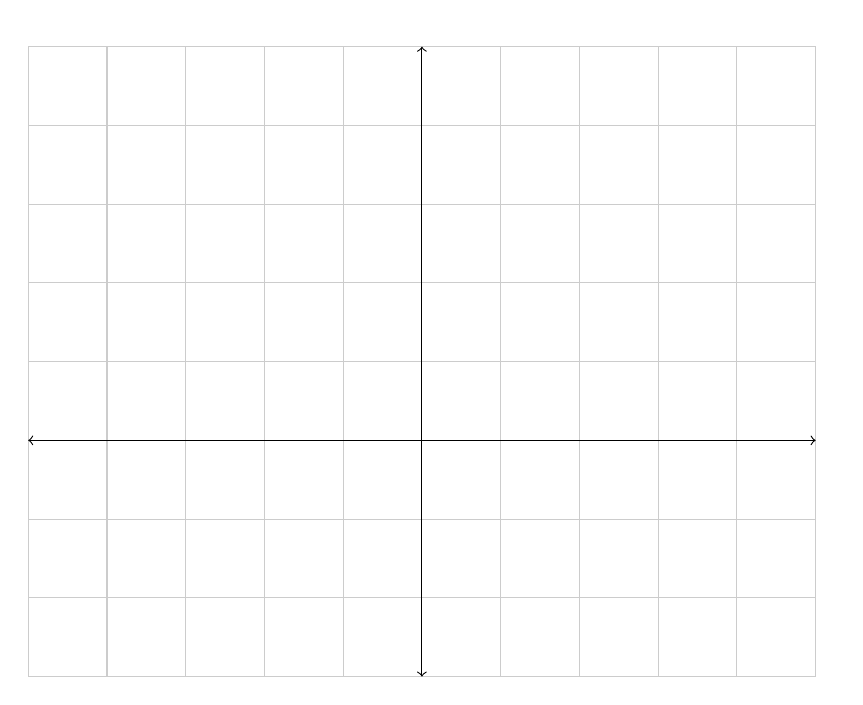
\begin{tikzpicture}[scale=1]
		        \draw[thin,gray!40] (-5,-3) grid (5,5);
		        \draw[<->] (-5,0)--(5,0) node[right]{$\RE$};
		        \draw[<->] (0,-3)--(0,5) node[above]{$\IM$};
		        \end{tikzpicture}
		  \]
	\item (\textbf{3 pts.}) Compute the norm of the function $\|f\|$ using the Hermitian inner product for the interval $[-4,4]$.
	\item 
\end{enumerate}
\end{problem}

\newpage
\emph{Intentionally left blank to be used as scratch paper.}\\


% Problem 3
\newpage
\begin{problem} Consider the linear differential equation $-\frac{d^2}{dx^2}f(x)=\omega^2f(x)$ where $\omega$ is a constant.
\begin{enumerate}[(a)]
	\item	(\textbf{3 pts.}) Suppose that both $f_1(x)$ and $f_2(x)$ are solutions. Show that $\alpha_1f_1(x)+\alpha_2 f_2(x)$ is also a solution.
	\item	(\textbf{3 pts.}) If we have that $f_n(x)$ is a solution for all \underline{integers} $n$, explain why 
	\[
	\Psi(x) = \sum_{n=-\infty}^\infty \alpha_n f_n(x),
	\]
	is also a solution.
	\item	(\textbf{3 pts.}) If indeed $f_k(x)$ is a solution for all \underline{real numbers} $k$, explain why 
	\[
	\Phi(x) = \int_{-\infty}^\infty f_k(x) dk,
	\]
	is also a solution.
	\item	(\textbf{3 pts.}) Show that the function 
	\[
	f_k(x) = e^{i2\pi kx},
	\]
	is a solution
	
	This isn't quite true. Well it is, but you find THE solution from the boundary conditions
\end{enumerate}
\end{problem}

\newpage
\emph{Intentionally left blank to be used as scratch paper.}\\


% Problem 4
\newpage
\begin{problem}
inner products, symmetry, hermitian
\end{problem}

\newpage
\emph{Intentionally left blank to be used as scratch paper.}\\


% Problem 5
\newpage
\begin{problem} 
 Fourier series
\end{problem}

\newpage
\emph{Intentionally left blank to be used as scratch paper.}\\


% Problem 6
\newpage
\begin{problem}
Fourier transforms, something with different boundary conditions. If eqn solves for one boundary condition, does it solve for another?
\end{problem}
\newpage
\emph{Intentionally left blank to be used as scratch paper.}\\

\end{document}  